\documentclass[11pt,a4paper]{article}

\usepackage[utf8]{inputenc}
\usepackage[T1]{fontenc}
\usepackage[english]{babel}
\usepackage[a4paper,margin=2.3cm]{geometry}
\usepackage{amsmath,amssymb}
\usepackage{graphicx}
\usepackage{booktabs}
\usepackage{caption}
\usepackage{float}
\usepackage[numbers,sort&compress]{natbib}
\usepackage{xcolor}
\usepackage{hyperref}
\graphicspath{{../figuras/}}
\captionsetup{font=small,labelfont=bf}

\title{\textbf{Predicting ATP Match Winners with Surface-Specific Elo Ratings\\and a Model Ensemble under Temporal Validation}}
\author{
  Juan Pablo Angonese, Agustín José Ceballos Pratto, Alan Yair Ghibaudo,\\
  Emanuel Genaro Scrosati, Genaro Villegas and Juan José Wendler\\[4pt]
  \small National Technological University, Regional Faculty of Córdoba, Argentina\\
  \small Data Science course project (5K2, 2026), group no.~4
}
\date{}

\begin{document}
\maketitle

\begin{abstract}
Predicting the winner of a professional tennis match is a problem with abundant data and results that are hard to anticipate. We use 70,311 ATP matches (2000--2026) to estimate the probability that one player beats another, using only information available before the match. The features describe each player's history: overall and surface-specific Elo ratings, recent form, serve and return statistics with exponential moving averages, head-to-head record, and the official ranking. We evaluate with a temporal split (training before 2024, test from 2024 to 2026) and with symmetric prediction to remove the arbitrary ordering of players. The ensemble of logistic regression, Random Forest and Gradient Boosting reaches 64.6\% accuracy and a ROC-AUC of 0.714 on the test set, compared with 63.7\% and 0.689 for the rule ``the higher-ranked player wins''. An ablation study shows that history alone, without the ranking, matches the full model, and that Elo is the most influential feature family. The probabilities are well calibrated: when the model assigns more than 90\% to the favourite, the favourite wins 94\% of the time. We also present a tournament simulator that explains the probability of each round. We discuss the limits of the approach, including the ceiling imposed by chance.
\end{abstract}

\noindent\textbf{Keywords:} sports prediction, tennis, Elo rating, temporal validation, calibration, machine learning.

\section{Introduction}

A professional tennis match pits two players with very different histories, surfaces and form. Predicting the winner is of interest to analysts, the media and coaching staff preparing an opponent. The usual shortcut is the official ranking, which summarises points accumulated over the last 52 weeks. This shortcut has two drawbacks: it penalises players returning from injury or competing less often, and it does not distinguish sustained performance from a recent spike.

This work asks whether a player's full history improves the prediction of the winner, and by how much. Our contributions are:
\begin{itemize}
  \item A documented cleaning and transformation process for a public ATP match database, with decisions justified by the distribution of each variable and by domain rules.
  \item An evaluation design that avoids information leakage: features computed only from earlier matches, a temporal split, and symmetric prediction.
  \item A set of history features (overall and surface Elo, form, serve, return, head-to-head) compared against the ranking through ablation and grouped permutation importance.
  \item A calibration analysis of the probabilities, a use case, and a tournament simulator.
\end{itemize}

\section{Related work}

The Elo system \cite{elo1978} estimates a player's strength from results and from the expected strength of opponents, updating after every match. It is the basis of our strength features. Kovalchik \cite{kovalchik2016} compares methods for predicting tennis matches, including ranking-based and match-statistics-based models.

We use three families of models: regularised logistic regression, Random Forest \cite{breiman2001} and Gradient Boosting \cite{friedman2001}. For feature importance we follow Breiman's permutation approach \cite{breiman2001}, grouping correlated variables. Validation respects temporal order, as recommended by Bergmeir and Benítez \cite{bergmeir2012}. To assess probability quality we use Log-Loss, the Brier score \cite{brier1950} and the ROC curve \cite{fawcett2006}, and we analyse calibration in the spirit of \cite{guo2017}.

\section{Data}

\subsection{Source and volume}

We use the TML-Database \cite{tml2026}, which compiles ATP circuit results from a scrape of the official source and from Sackmann's open datasets \cite{sackmann}. The match table has 78,091 records between 2000 and 2026, with 50 columns: tournament, surface, level, round, data for both players, score, duration and serve and return statistics. The player table provides date of birth, height and handedness. We join both tables on the player identifier and keep 2,733 players active in the period.

\subsection{Data quality}

Table~\ref{tab:quality} summarises the state before and after treatment. There are no exact duplicate rows. Missing values in the match table drop from 378,735 to zero.

\begin{table}[H]
\centering
\caption{Data quality before and after treatment.}
\label{tab:quality}
\begin{tabular}{lrr}
\toprule
Metric & Before & After \\
\midrule
Matches (rows) & 78,091 & 70,311 \\
Duplicate rows & 0 & 0 \\
Missing values in matches & 378,735 & 0 \\
Columns in matches & 50 & 59 \\
Players (rows) & 7,643 & 2,733 \\
Missing values in players & 38,254 & 109 \\
\bottomrule
\end{tabular}
\end{table}

Missing statistics are not uniform. Davis Cup and the Olympics have 80.1\% and 57.8\% of matches without playing statistics, and they follow a different format from the tour. We exclude them (Figure~\ref{fig:nulls}). In the remaining levels, missing values are below 1\%.

\begin{figure}[H]
\centering
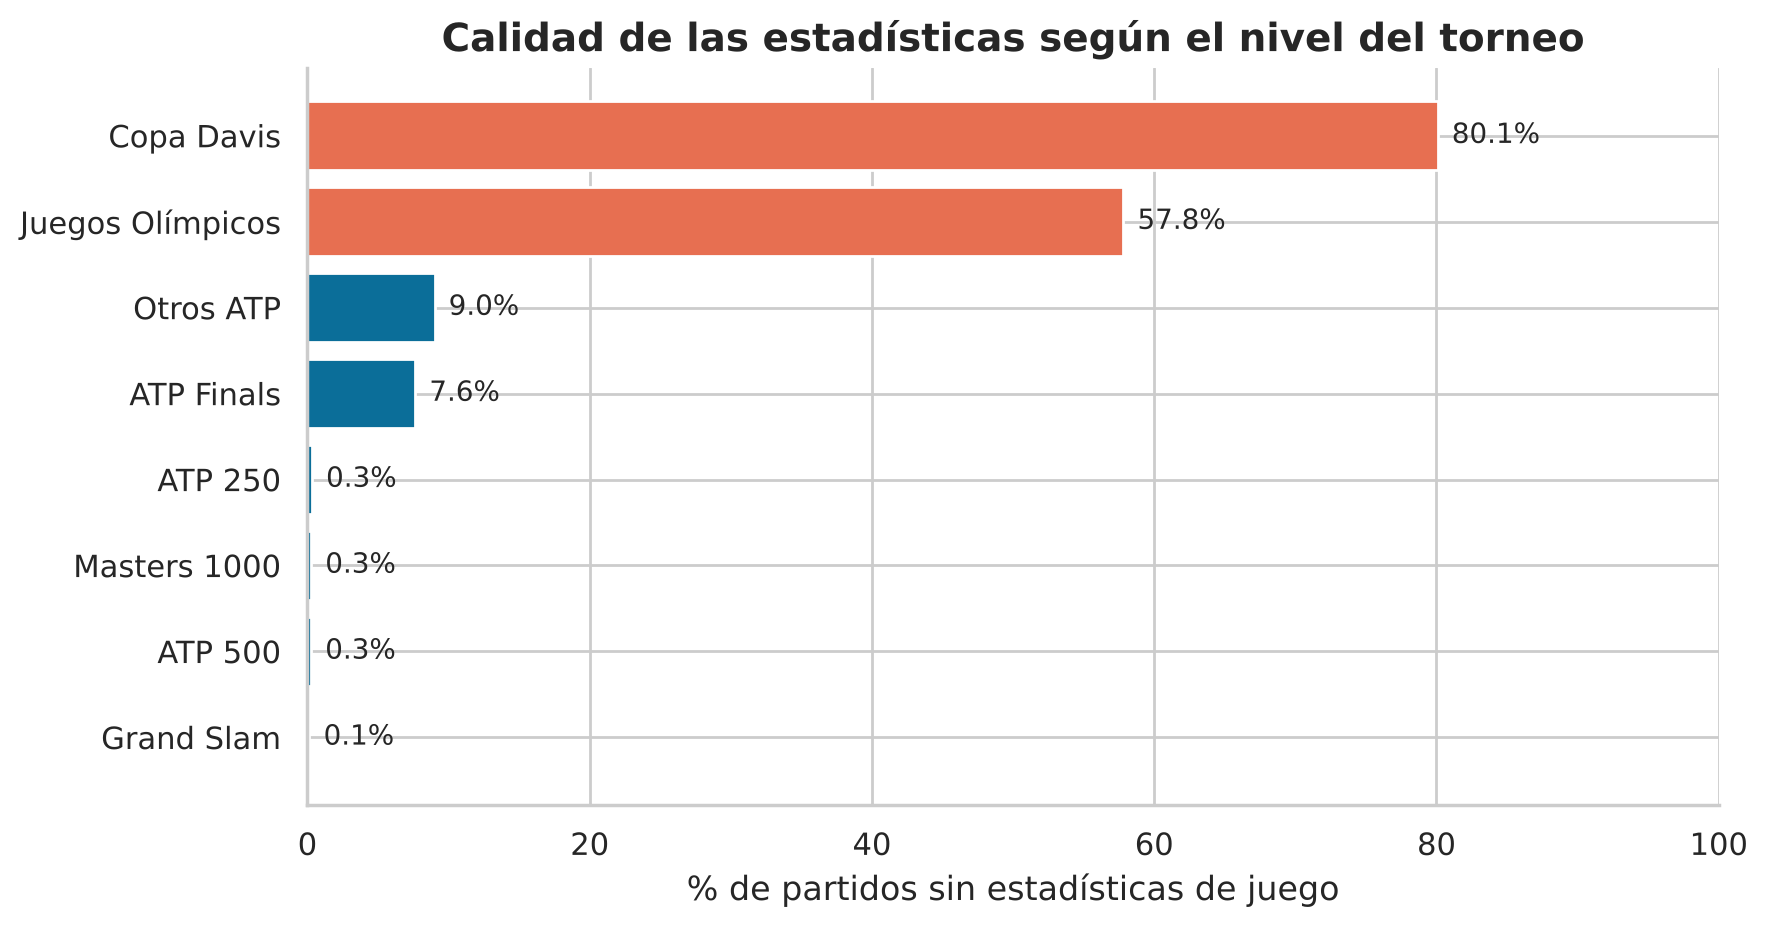
\includegraphics[width=0.8\linewidth]{fig02_nulos_por_nivel.png}
\caption{Share of matches without playing statistics by tournament level. Levels in orange are excluded.}
\label{fig:nulls}
\end{figure}

For outliers in duration and height we do not apply mass removal, since a long match is a real event. Imputations depend on distribution: the median for height and age, which are symmetric; the median by set format for duration, which has a long right tail; and the median by surface for missing statistics. Figure~\ref{fig:outliers} shows the distribution before and after.

\begin{figure}[H]
\centering
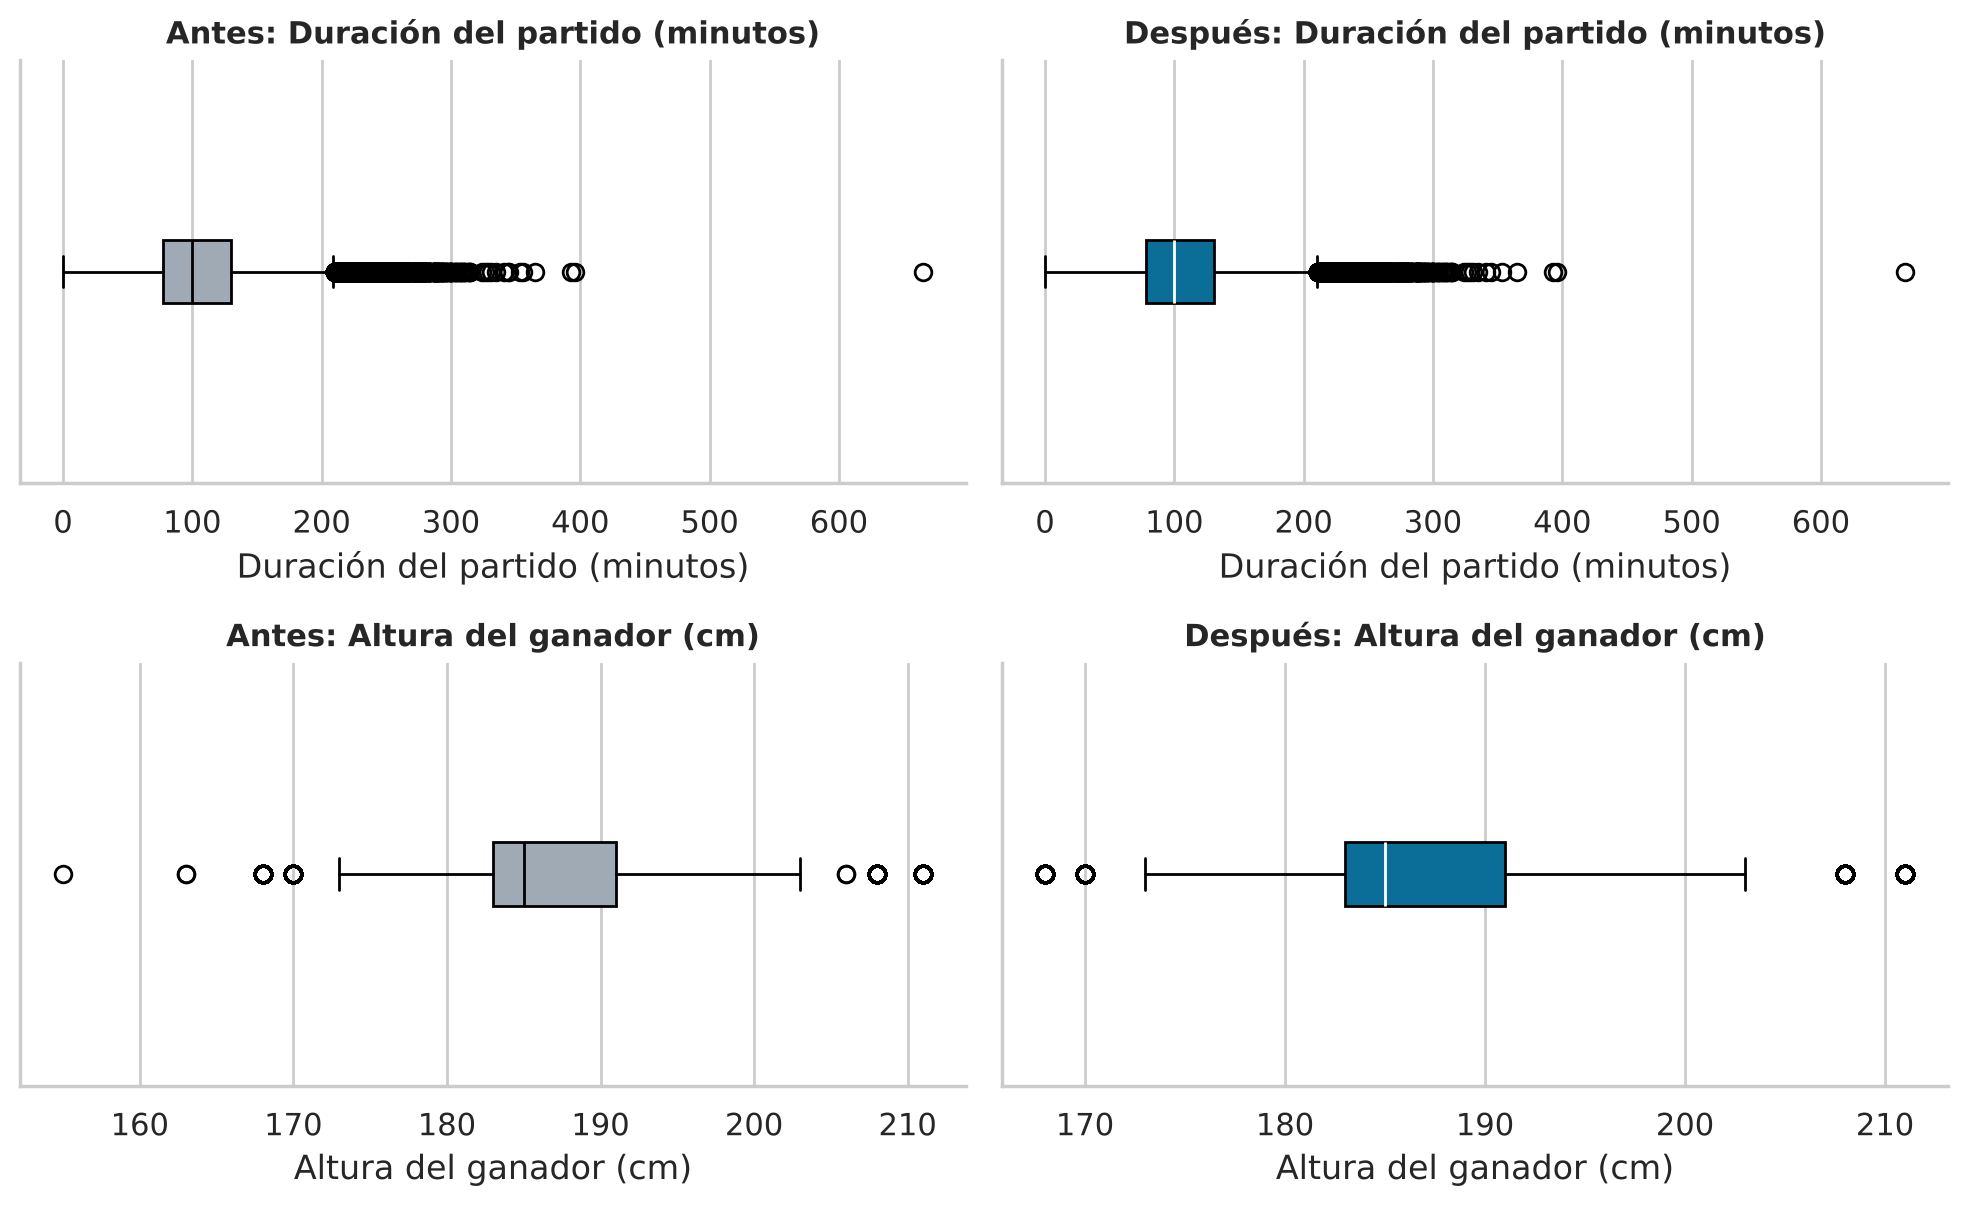
\includegraphics[width=0.85\linewidth]{fig11_pre_post_outliers.png}
\caption{Outliers in match duration and winner height, before (left) and after (right) treatment.}
\label{fig:outliers}
\end{figure}

\section{Methods}

\subsection{Features}

We build 73 predictor features in eight families (Table~\ref{tab:families}). For each player, features are computed from matches played before the match being predicted; the match's own statistics never enter the model.

\begin{table}[H]
\centering
\caption{Predictor feature families.}
\label{tab:families}
\begin{tabular}{p{4.2cm}p{7.5cm}}
\toprule
Family & What it describes \\
\midrule
ATP ranking & Official position and points \\
Elo, overall and by surface & Underlying strength, updated after each result \\
Recent form & Wins in the last 10 matches \\
Surface & Share of wins on the match surface \\
Serve & Serve effectiveness (exponential moving average) \\
Return & Points won on return and break points converted \\
Head-to-head & Previous wins between the two players \\
Physical and activity & Age, height, experience and days since last match \\
\bottomrule
\end{tabular}
\end{table}

Absolute counts (aces, serve points) depend on match length, so we use percentages. Statistics are averaged with an exponential moving average of window 20, to reflect current level rather than a past peak.

\subsection{Elo rating}

Each player starts at 1,500. After each match, the winner gains and the loser loses:
\begin{equation}
  E = \frac{1}{1 + 10^{(R_{\text{opp}} - R_{\text{player}})/400}}, \qquad R \leftarrow R + K\,(S - E),
\end{equation}
where $S=1$ for a win and $S=0$ for a loss, and the adjustment factor is $K = 250/(n+5)^{0.4}$, with $n$ the number of matches played. A new player adjusts quickly and a veteran stabilises. Walkovers do not update the rating. We compute an overall Elo and a surface-specific Elo.

\subsection{Chronological order and symmetry}

All matches of a tournament share the start date. To avoid a final appearing before earlier matches, we sort by date, tournament, round and match number. Each match is represented symmetrically: we randomly assign which player is A (fixed seed). Prediction is made in both directions (A against B and B against A) and averaged, so the result does not depend on ordering. The positive class is balanced (50\%).

\subsection{Temporal split and validation}

We train on 64,729 matches before 1 January 2024 (92.1\%) and evaluate on 5,582 matches from that date to 17 January 2026 (7.9\%). We do not use a random split: with temporal data it would allow training on matches that occur after those being predicted. Hyperparameter search uses five-fold temporal cross-validation, which always trains on the past and validates on the following period.

\subsection{Models and hyperparameters}

We compare four models against a domain baseline, the rule ``the higher-ranked player wins''. Table~\ref{tab:models} lists the selected hyperparameters and cross-validated Log-Loss. Selection used Log-Loss because the models output probabilities and this metric penalises overconfident predictions.

\begin{table}[H]
\centering
\caption{Candidate models, selected hyperparameters and temporal cross-validated Log-Loss (lower is better).}
\label{tab:models}
\begin{tabular}{llp{4.6cm}r}
\toprule
Model & Core idea & Selected hyperparameters & Log-Loss \\
\midrule
Logistic regression & Weighted sum, mapped to probability & $C=0.01$ (L2 regularisation) & 0.5907 \\
Random Forest & Parallel trees, majority vote & 150 trees, depth 14, minimum 20 matches per leaf & 0.5935 \\
Gradient Boosting & Sequential trees correcting errors & Learning rate 0.03, depth 3, minimum 100 matches per leaf & 0.5916 \\
Ensemble (average) & Average of the three above & -- & \textbf{0.5901} \\
\bottomrule
\end{tabular}
\end{table}

The ensemble has the lowest cross-validated Log-Loss. Its difference from logistic regression is small (0.0006), smaller than the variability across temporal folds (about 0.0125). The ensemble's advantage is real but modest.

\subsection{Metrics}

We use accuracy, ROC-AUC, Log-Loss,
\begin{equation}
  \text{Log-Loss} = -\frac{1}{N}\sum_{i=1}^{N}\big[y_i\log p_i + (1-y_i)\log(1-p_i)\big],
\end{equation}
and the Brier score, $\frac{1}{N}\sum_i (p_i - y_i)^2$. With the symmetrised target, precision, recall and F1 almost coincide with accuracy: a false positive and a false negative are the same error, namely choosing the player who lost. We therefore do not use them as the main criterion.

\section{Results}

\subsection{Test performance}

Table~\ref{tab:results} compares the final model with the baseline on the 5,582 test matches.

\begin{table}[H]
\centering
\caption{Test performance (2024--2026).}
\label{tab:results}
\begin{tabular}{lrr}
\toprule
Metric & Baseline (ranking) & Final model \\
\midrule
Accuracy & 63.7\% & \textbf{64.6\%} \\
ROC-AUC & 0.689 & \textbf{0.714} \\
Log-Loss & -- & \textbf{0.6166} \\
Brier & -- & \textbf{0.2148} \\
\bottomrule
\end{tabular}
\end{table}

Figure~\ref{fig:comparison} compares the models. The four individual models are very close to one another, and all of them beat the ranking. This suggests that information matters more than the algorithm. Figure~\ref{fig:confusion} shows the confusion matrix of the final model. Because of symmetrisation, the ``wins A / wins B'' axis has no special meaning: the diagonal is what matters.

\begin{figure}[H]
\centering
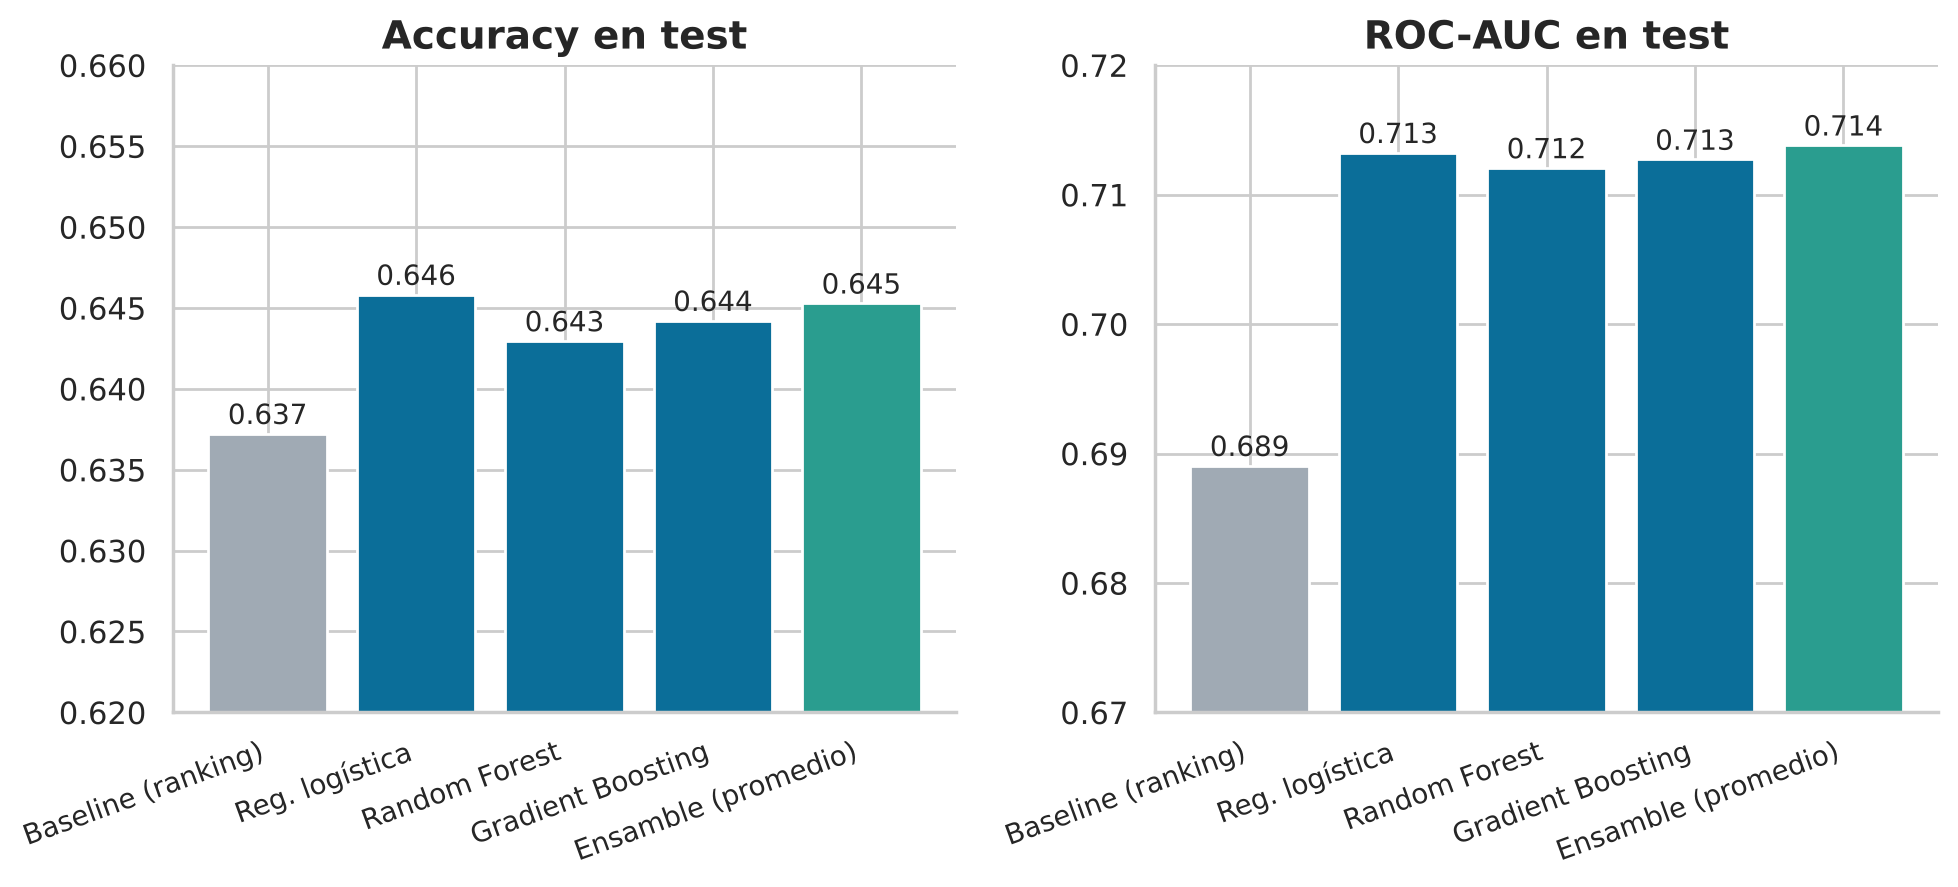
\includegraphics[width=0.85\linewidth]{fig04_comparacion_modelos.png}
\caption{Accuracy and ROC-AUC on the test set. Grey: ranking baseline; blue: individual models; green: final model. Axes do not start at zero.}
\label{fig:comparison}
\end{figure}

\begin{figure}[H]
\centering
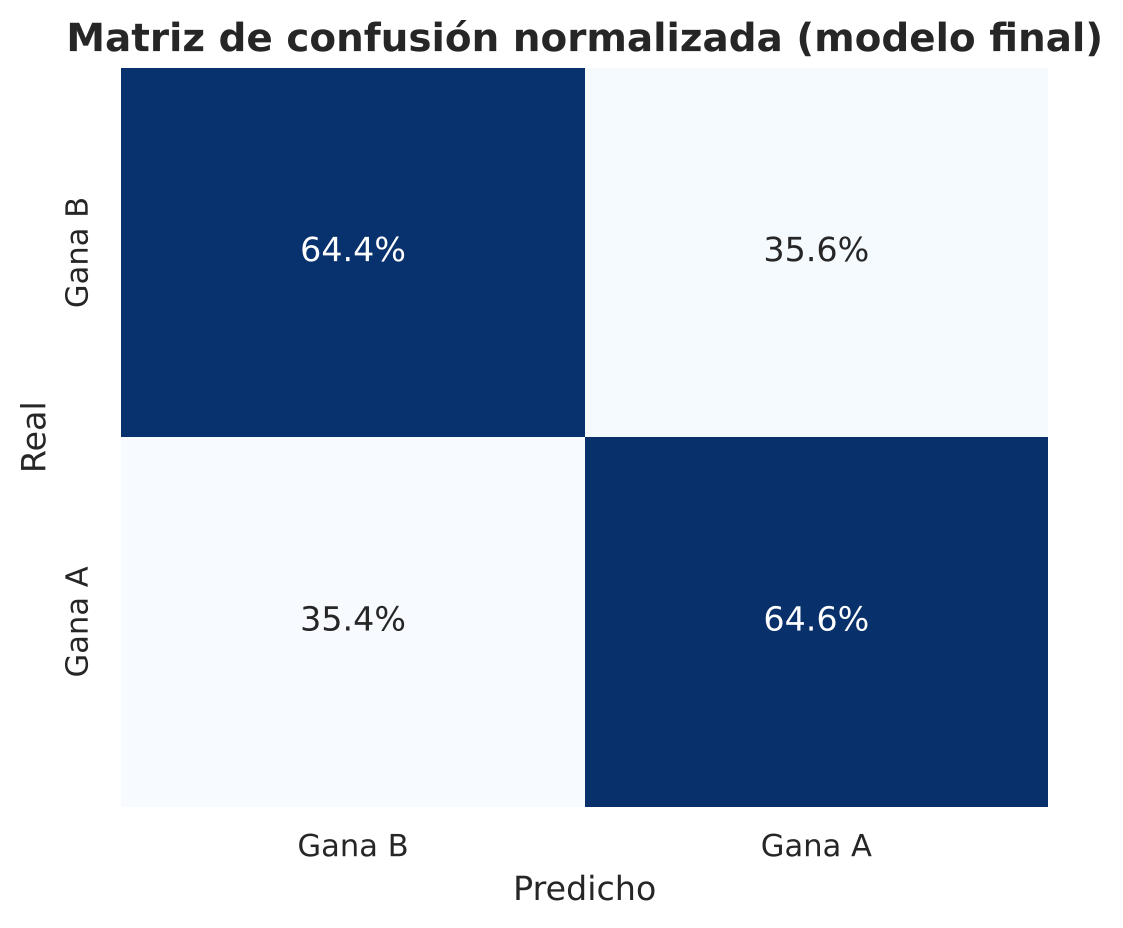
\includegraphics[width=0.55\linewidth]{fig10_matriz_confusion.png}
\caption{Row-normalised confusion matrix of the final model on the test set.}
\label{fig:confusion}
\end{figure}

\subsection{Calibration of probabilities}

We group test matches by the model's confidence in the favourite (Figure~\ref{fig:calibration}). In the 90--100\% bin (198 matches), the model predicted 92.9\% and the favourite won 94.4\%. In matches between top-10 players (120 matches), the model assigned 67.1\% on average and the favourite won 70.8\%. In the intermediate bins, the gap between predicted and observed is 2 to 3 points, with the model slightly optimistic. For clear favourites, the model is slightly conservative. Overall, the probabilities are reasonably reliable, though not perfect.

\begin{figure}[H]
\centering
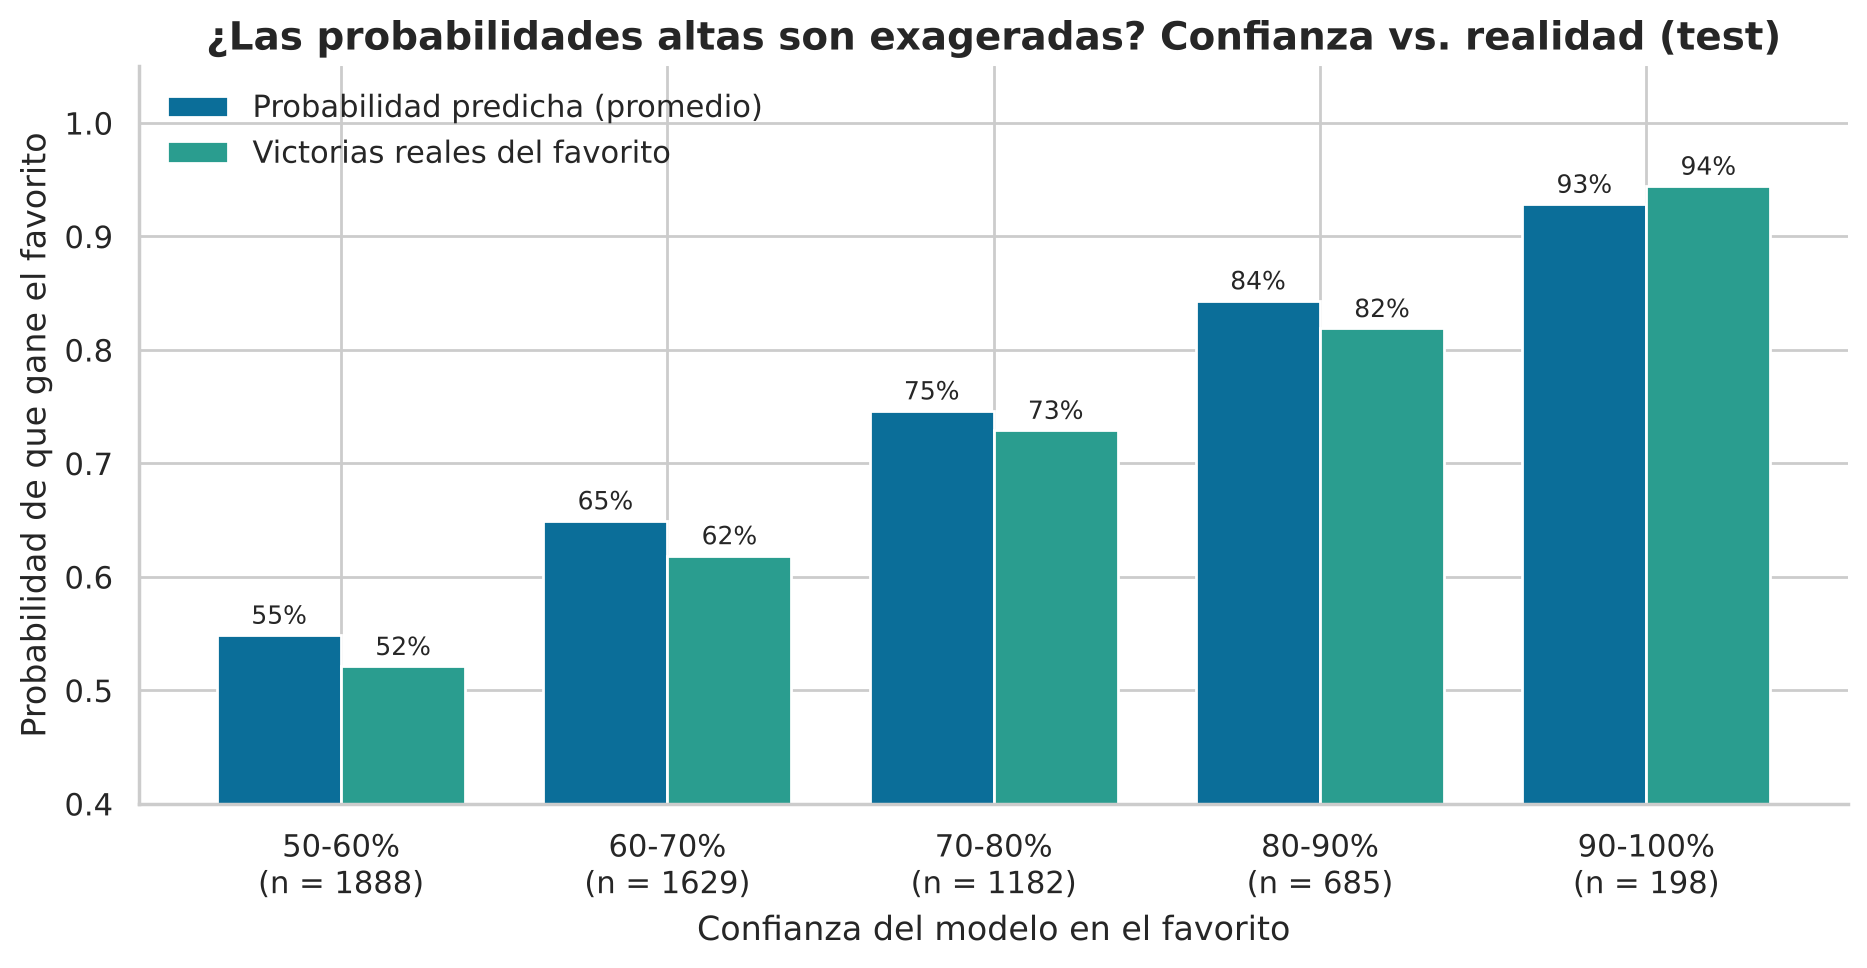
\includegraphics[width=0.8\linewidth]{fig06_calibracion_confianza.png}
\caption{Model confidence in the favourite versus observed win frequency on the test set. Equal bar heights indicate good calibration.}
\label{fig:calibration}
\end{figure}

\subsection{Ablation: does the model only use the ranking?}

We train three versions: ranking only (9 features), history without ranking (65 features) and full (73 features). Figure~\ref{fig:ablation} shows the results. The model without ranking reaches 64.6\% accuracy (ROC-AUC 0.711), practically the same as the full model (64.7\%; 0.713) and better than ranking alone (63.3\%; 0.690). The history carries the relevant information, and the ranking is a partial summary of it.

\begin{figure}[H]
\centering
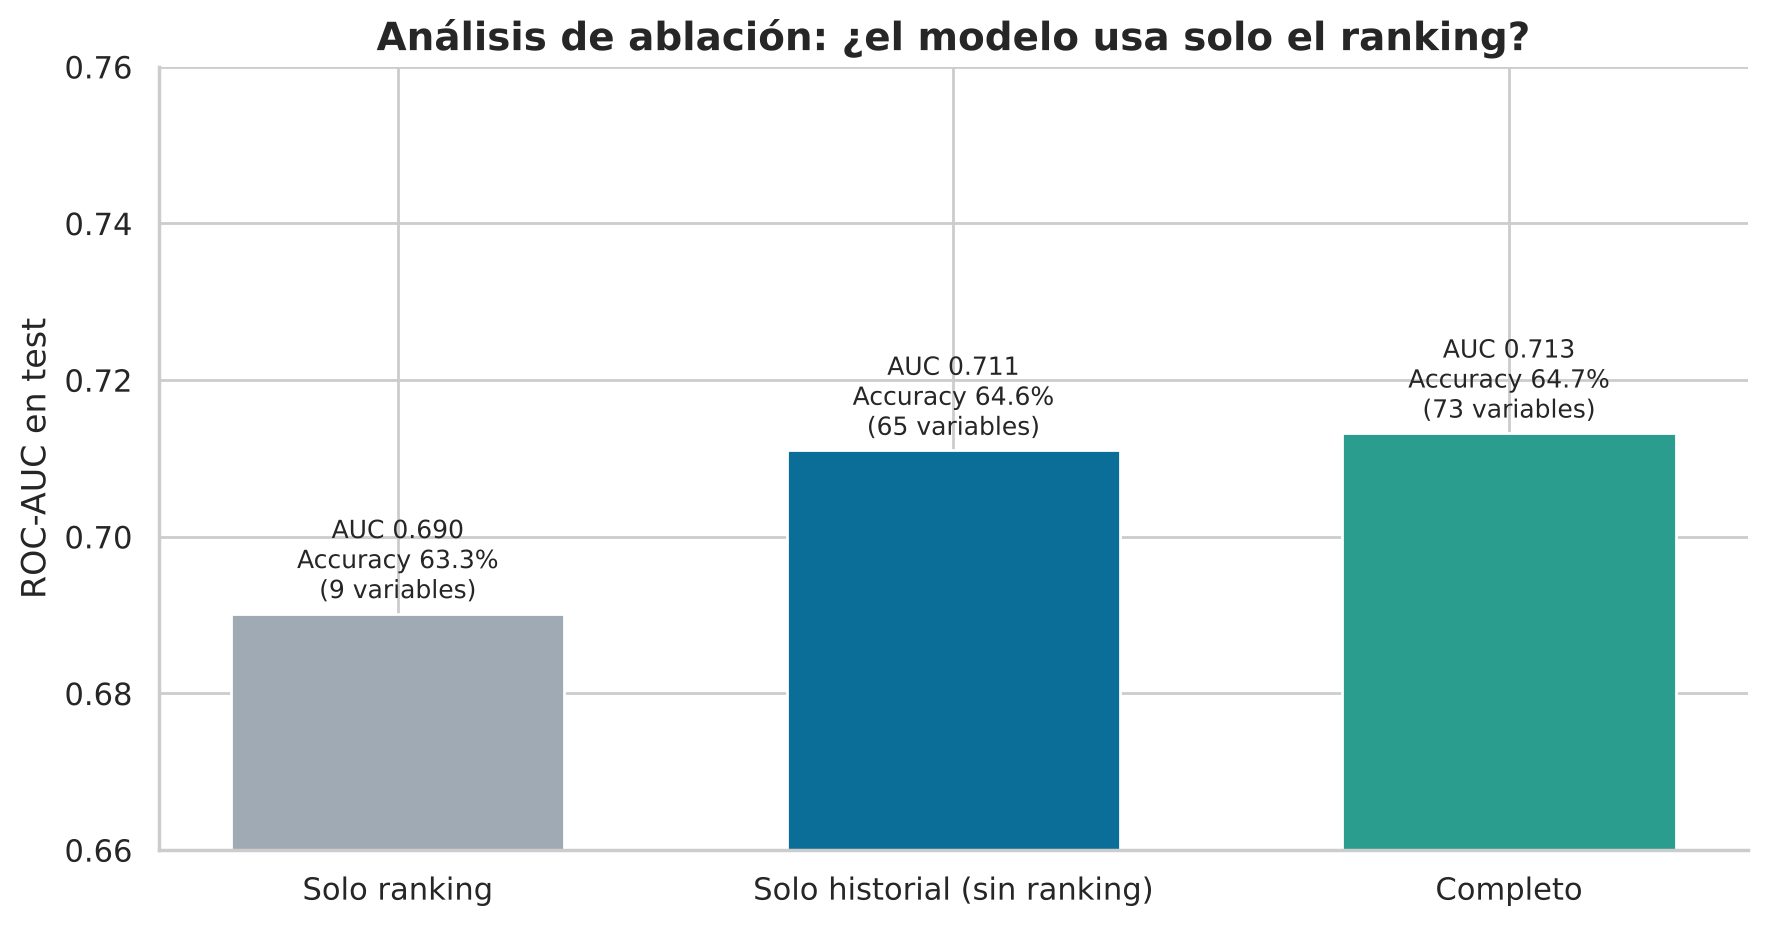
\includegraphics[width=0.8\linewidth]{fig07_ablacion.png}
\caption{ROC-AUC on the test set by feature set.}
\label{fig:ablation}
\end{figure}

\subsection{Feature family importance}

We measure importance by grouped permutation: we shuffle all features of one family together and record the drop in test ROC-AUC (mean of five repetitions on 4,000 matches). Grouping is necessary because Elo and ranking points are strongly correlated: shuffling one alone would be compensated by the other, making both look unimportant.

Overall and surface Elo drops by 0.066, almost four times the drop for the ranking (0.018). Recent serve (0.010) and the physical and activity block (0.007) follow. Last-10-match form (0.0001) and head-to-head (0.0006) add little once the model has finer form measures (Figure~\ref{fig:importance}).

\begin{figure}[H]
\centering
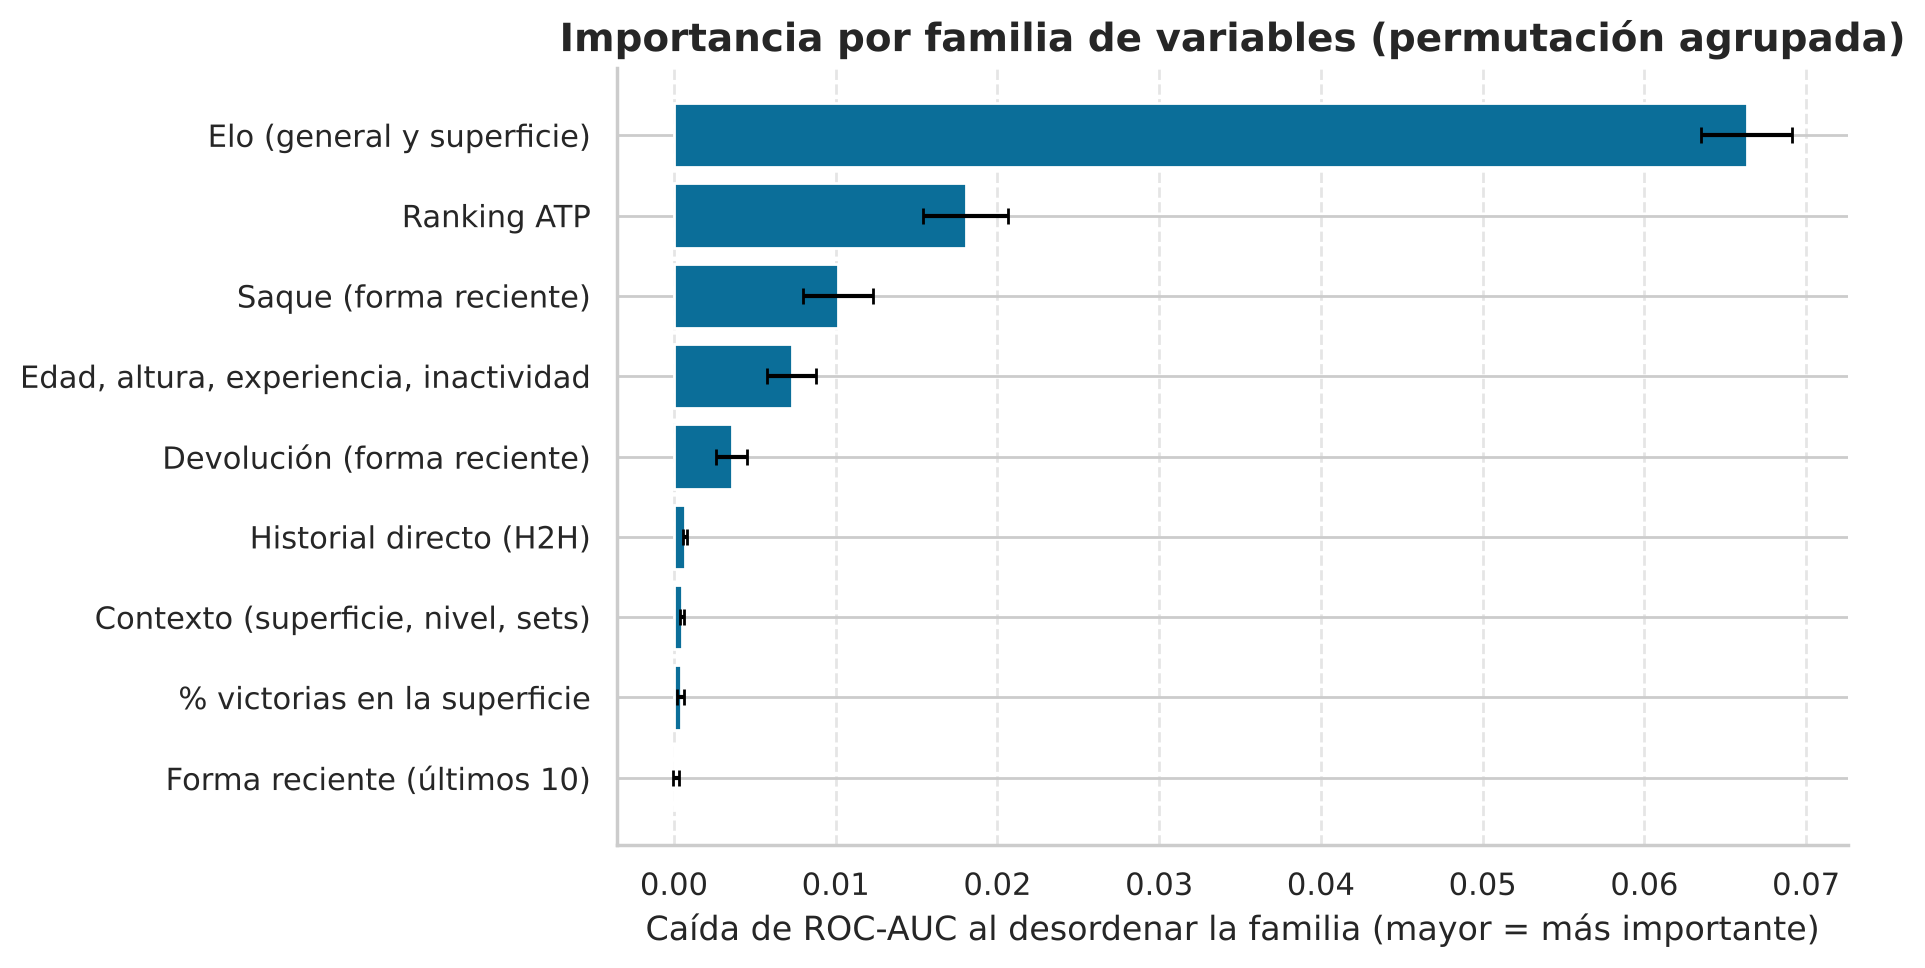
\includegraphics[width=0.8\linewidth]{fig08_importancia_familias.png}
\caption{Feature family importance: drop in test ROC-AUC when the family is shuffled (black bars: standard deviation).}
\label{fig:importance}
\end{figure}

\subsection{Performance by context}

Figure~\ref{fig:context} compares the model with the ranking by surface, tournament level and ranking gap. Results are heterogeneous. On grass, the model improves on the ranking by 3.4 points (66.5\% versus 63.1\%). On clay and hard courts, the gain is small. At Grand Slams, the model reaches 72.7\% versus 70.2\%. At Masters 1000, the ranking is better (63.8\% for the model versus 64.9\%). When the ranking gap exceeds 250 places, the ranking is more accurate (67.7\% versus 66.1\%). Levels with small samples, such as ATP Finals (30 matches), are not interpreted.

\begin{figure}[H]
\centering
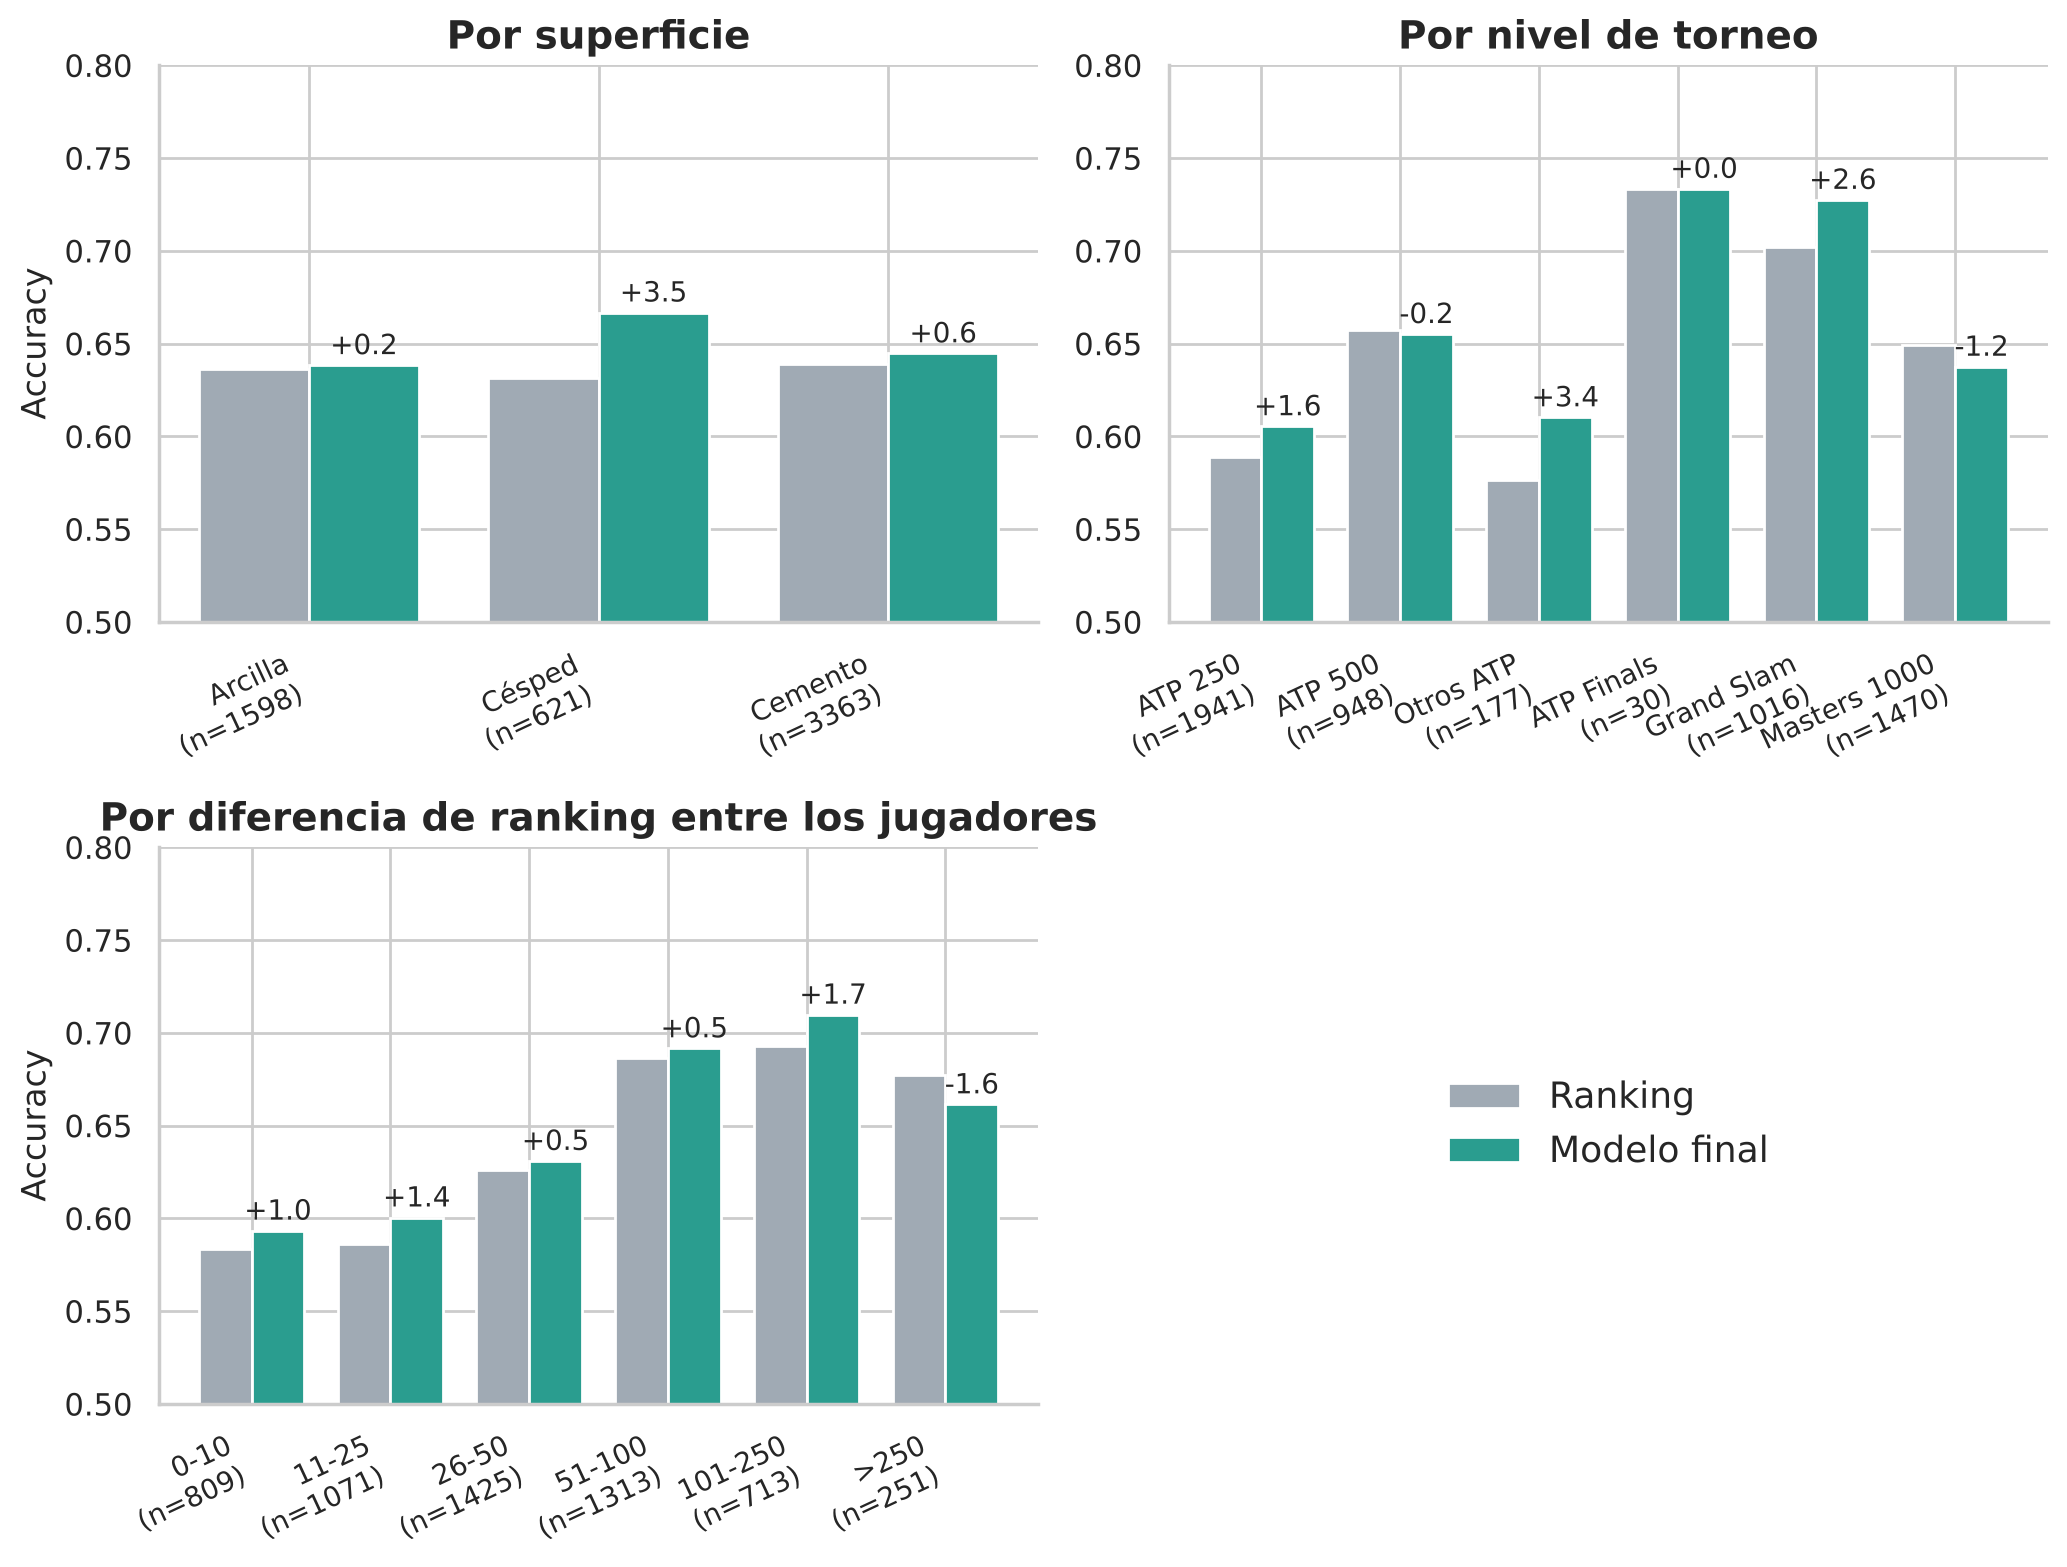
\includegraphics[width=0.95\linewidth]{fig09_accuracy_por_contexto.png}
\caption{Accuracy of the ranking (grey) and the final model (green) by surface, tournament level and ranking gap. Numbers show the difference in percentage points.}
\label{fig:context}
\end{figure}

\subsection{Use case}

As an example, consider a clay-court match between Holger Rune (ranking 11, clay Elo 1,917) and Valentin Vacherot (ranking 32, clay Elo 1,448). The model assigns 75.5\% to Rune. The family-level explanation attributes most of this gap to overall and surface Elo (+15.7 points), followed by recent return (+3.0) and ranking (+2.9). This case shows how the model reaches its number; it does not validate the model by itself. We also simulate an eight-player draw and a 32-player draw of randomly chosen active players, reporting each round's probability and the variables that explain it.

\section{Discussion}

\textbf{What worked.} Combining surface-specific Elo, serve and return statistics with exponential moving averages captures a player's current level better than the official ranking. Temporal validation and symmetric prediction gave an honest evaluation: results do not depend on the arbitrary ordering of players or on data posterior to the match.

\textbf{What did not work as well.} The algorithm matters little compared with the information: the four models are very close. The advantage over the ranking is moderate (0.9 accuracy points and 0.025 ROC-AUC). When ranking gaps are very large, the ranking is already sufficient.

\textbf{Limits.} Chance imposes a ceiling: about 36\% of test matches are won by the lower-ranked player. The model does not include injuries, fatigue, weather or market odds. Context differences do not yet have statistical significance tests, and levels with few matches should be read with caution.

\section{Areas for improvement}

These items fall outside the results presented here. They are proposals for a next iteration.

\begin{itemize}
  \item \textbf{Retraining alternatives.} We did not evaluate weighting recent matches or limiting the history to matches from 2010 onwards. Both could improve the estimate of players' current form.
  \item \textbf{Market odds.} Odds summarise public information available before the match. Incorporating them is a proposal; this work reports no figures for it.
  \item \textbf{Injuries and fatigue.} These are relevant factors that are not in the database today.
  \item \textbf{Performance evolution.} The trajectory of each player across a career, planned at the project stage, remains pending.
  \item \textbf{Statistical significance.} Context differences, such as the Grand Slam one, should be tested on the same matches (for example, with McNemar's test).
  \item \textbf{Tournament simulation.} Estimating the probability of winning a title requires simulating thousands of draws, not a single scenario. In addition, the 32-player draw uses a three-set format for a Grand Slam; the format should be unified.
\end{itemize}

\section{Conclusions}

Predicting the winner of a professional tennis match using only information available before the match is possible, with a moderate gain over the ranking. The player's history, in particular surface-specific Elo, contributes the relevant information. The model's probabilities are reasonably reliable, especially for clear favourites. Chance is the main obstacle, and any pre-match prediction faces it. We do not recommend using the model for betting: its advantage over the ranking is small and has not been validated against real odds.

\section*{Code and data availability}

The code and the notebook with outputs are at \url{https://github.com/genavillegas/atp-match-prediction}, under the MIT licence. The file \texttt{requirements.txt} pins the library versions with which we reproduced the notebook (scikit-learn 1.6.1, pandas 2.2.2, numpy 2.0.2). With these versions, logistic regression and Random Forest match the reported values; Gradient Boosting differs in a few predictions near the threshold, so the ensemble's accuracy may read 64.5\% instead of 64.6\%. The data come from the TML-Database \cite{tml2026} and are not included in the repository; they should be consulted under their original licence.

\bibliographystyle{plainnat}
\bibliography{refs}

\end{document}
